\documentclass{beamer}
\usepackage{graphicx,amsmath,amsfonts,amssymb,listings,tikz}
\usepackage{multimedia}
\usetheme{Montpellier}
\usecolortheme{beaver}
\beamerdefaultoverlayspecification{<+->}
\definecolor{mygray}{rgb}{0.92,0.92,0.92}

% user commands
\newcommand{\weeknum}{9}

\begin{document}

\section{Introduction}
\title{A Multiresolution Scheme for More Efficient Simulation on Adaptive Mesh Refinement Blocks?}
\author{Brandon Gusto} %
\institute{Dept. of Scientific Computing \\ Florida State University}
\date{\today}
\frame{\titlepage}

\section{Introduction}

\begin{frame}{Introduction}
    The following project is concerned with the numerical solution of systems of conservation laws of the form
    \begin{equation*}
        \mathbf{U}_{t} + \mathbf{F}(\mathbf{U})_{x} = 0
    \end{equation*}
    where $\mathbf{U} = (\rho,\rho u,E)$ is a vector of conserved quantities and $\mathbf{F}(\mathbf{U})$ is a flux vector.
    Consider a standard finite-volume discretization, with midpoint rule
    \begin{equation*}
        \frac{\partial \mathbf{U}_{i}}{\partial t} = -\frac{1}{h} \left( \mathbf{F}_{i+\frac{1}{2}}
            - \mathbf{F}_{i-\frac{1}{2}} \right)
    \end{equation*}
    where the $i$ denotes spatial index.
\end{frame}

\begin{frame}{Adaptivity}
    The interest is in solution-adaptive methods:
    \begin{itemize}
        \item<2-> adaptive mesh refinement (AMR) based on local truncation error (or some other estimator)
        \item<3-> computations typically done on blocks / patches for efficiency
        \item<4-> inherent ``overresolution" in some regions of the mesh by using blocks
        \item<5-> can this be addressed by reducing block size? computational tradeoff?
    \end{itemize}
\end{frame}

\begin{frame}{AMR}
    \begin{figure}
        \center
        \includegraphics[scale=0.4]{amr1.png}
    \end{figure}
    \footnote{Introduction to Block-Structured Adaptive Mesh Refinement (AMR), Ann S. Almgren}
\end{frame}

\begin{frame}{AMR}
    \begin{figure}
        \center
        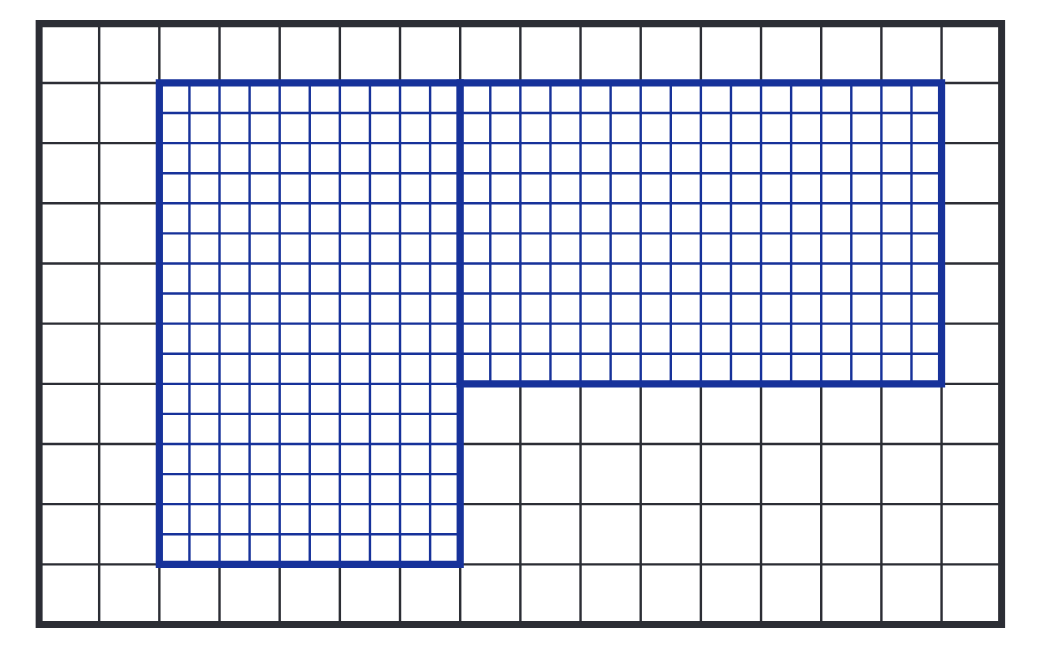
\includegraphics[scale=0.4]{amr2.png}
    \end{figure}
\end{frame}

\begin{frame}{AMR}
    \begin{figure}
        \center
        \includegraphics[scale=0.4]{amr3.png}
    \end{figure}
\end{frame}

\begin{frame}{Filling}
    The filling factor is the number of cells in a block which were flagged, divided by the total.
    \begin{figure}
        \center
        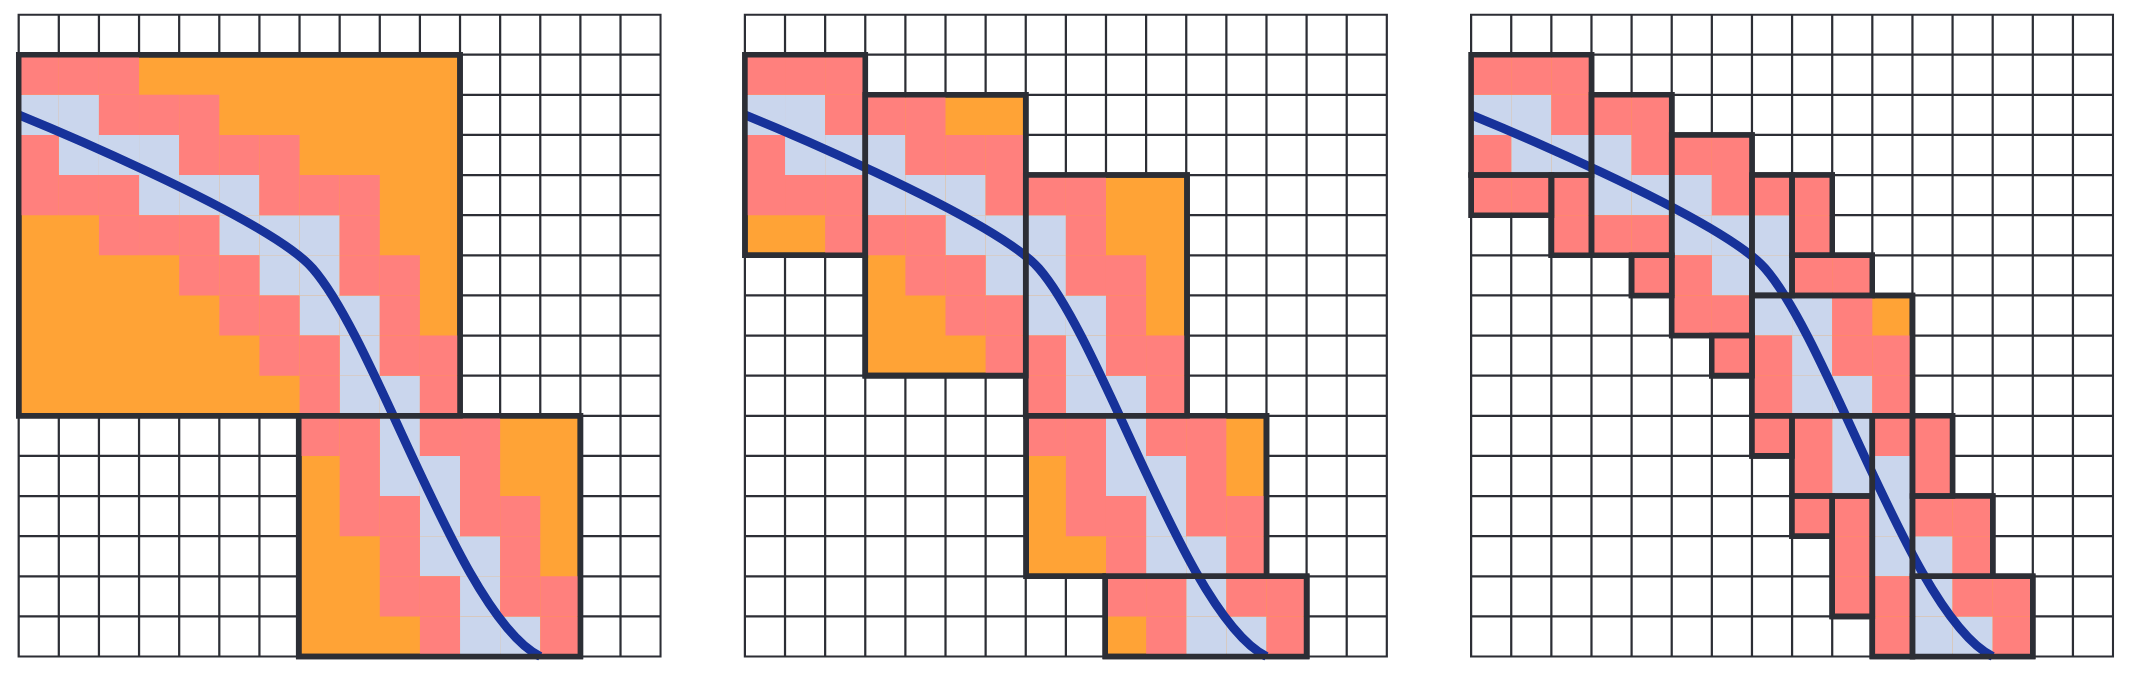
\includegraphics[scale=0.3]{filling.png}
    \end{figure}
\end{frame}

\section{Multiresolution}

\begin{frame}{a la Harten}
    \begin{itemize}
        \item<1-> Besides the AMR concepts, a multiresolution approach was also introduced by
            Harten. Grid is \textit{not} refined in space. Instead, a wavelet
            transform is performed on the uniform grid, and the fluxes are 
            interpolated in smooth regions. \\
        \item<2->``The goal of a multi-scale decomposition of a discrete set of
            data is a "rearrangement" of its information content in such a way
            that the new discrete representation, exactly equivalent to the old
            one, is more "manageable" in some respects." - Arandiga, Donat
    \end{itemize}
\end{frame}

\begin{frame}{Multiresolution}
    Define multiple, nested grids
    \begin{equation*}
        \mathbf{G}^{l} = \left\{ x^{l}_{i+\frac{1}{2}} \right\}_{i=0}^{N_{l}} =
            \left\{ x^{l+1}_{i+\frac{1}{2}} \right\}_{i=0,\text{i even}}^{N^{l+1}}.
    \end{equation*}
    Coarsening of avarage data in cell done via
    \begin{equation*}
        \mathbf{U}^{l}_{i} = \frac{1}{2} \left( \mathbf{U}^{l+1}_{2i} + \mathbf{U}^{l+1}_{2i+1} \right)
    \end{equation*}
\end{frame}

\begin{frame}{Decomposition}
    The prediction from coarse to fine is done by
    \begin{equation*}
        \mathbf{\hat{U}}^{l+1}_{2i+1} = \sum_{j=1-s}^{s-1} \gamma_{j} \mathbf{U}^{l}_{i+j}
    \end{equation*}
    The regularity information is assessed by computing detail coefficients as
    \begin{equation*}
        \mathbf{d}^{l}_{i} = \mathbf{U}^{l+1}_{2i+1} - \mathbf{\hat{U}}^{l+1}_{2i+1}.
    \end{equation*}
    A mask $\left\{ \mathbf{m} \right\}_{i}^{N^{l}}$ is created for significant cells.
\end{frame}

\begin{frame}{Decomposition}
    \begin{figure}
        \center
        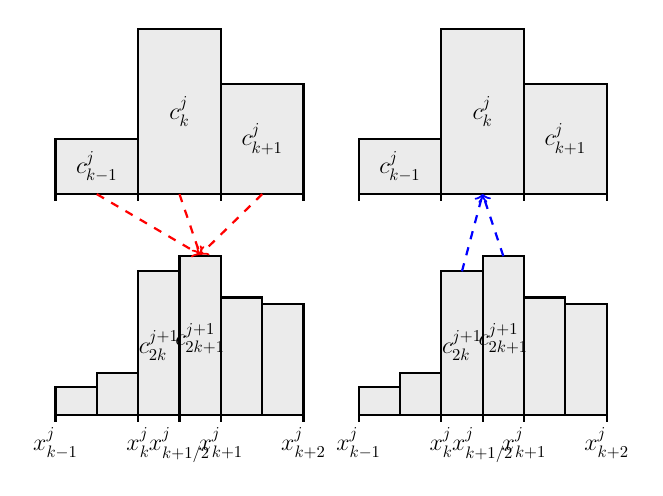
\begin{tikzpicture}[thick,scale=0.35, every node/.style={scale=0.6}]

        % variables
        \def\x{-8.0}
        \def\y{0.0}
        \def\yl{-8.0}

        % draw coarse level rectangles
        \draw [fill=mygray] (\x,0) rectangle (\x+3,2);
        \draw [fill=mygray] (\x+3,0) rectangle (\x+6,6);
        \draw [fill=mygray] (\x+6,0) rectangle (\x+9,4);

        % coarse level symbols
        \node at (\x+1.5,1) {\Large $c^{j}_{k-1}$};
        \node at (\x+4.5,3) {\Large $c^{j}_{k}$};
        \node at (\x+7.5,2) {\Large $c^{j}_{k+1}$};

        % coarse level axis
        \draw (\x,0) -- (\x,-0.25);
        \draw (\x+3,0) -- (\x+3,-0.25);
        \draw (\x+6,0) -- (\x+6,-0.25);
        \draw (\x+9,0) -- (\x+9,-0.25);

        % fine level rectangles
        \draw [fill=mygray] (\x,\yl) rectangle (\x+1.5,\yl+1);
        \draw [fill=mygray] (\x+1.5,\yl) rectangle (\x+3,\yl+1.5);
        \draw [fill=mygray] (\x+3,\yl) rectangle (\x+4.5,\yl+5.2);
        \draw [fill=mygray] (\x+4.5,\yl) rectangle (\x+6,\yl+5.75);
        \draw [fill=mygray] (\x+6,\yl) rectangle (\x+7.5,\yl+4.25);
        \draw [fill=mygray] (\x+7.5,\yl) rectangle (\x+9,\yl+4.0);

        % fine level symbols
        \node at (\x+3.75,\yl+2.5) {\Large $c^{j+1}_{2k}$};
        \node at (\x+5.25,\yl+2.75) {\Large $c^{j+1}_{2k+1}$};

        % fine level axis
	    \draw (\x,\yl) -- (\x,\yl-0.25);
        \draw (\x+3,\yl) -- (\x+3,\yl-0.25);
        \draw (\x+4.5,\yl) -- (\x+4.5,\yl-0.25);
        \draw (\x+6,\yl) -- (\x+6,\yl-0.25);
	    \draw (\x+9,\yl) -- (\x+9,\yl-0.25);

        % arrows
        \draw[red,dashed,->] (\x+1.5,\y) -- (\x+5.25,\y-2.20);
        \draw[red,dashed,->] (\x+4.5,\y) -- (\x+5.25,\y-2.20);
        \draw[red,dashed,->] (\x+7.5,\y) -- (\x+5.25,\y-2.20);

        % tick text
        \node[below] at (\x,\yl-0.25) {\Large $x^{j}_{k-1}$};
        \node[below] at (\x+3,\yl-0.25) {\Large $x^{j}_{k}$};
        \node[below] at (\x+4.5,\yl-0.25) {\Large $x^{j}_{k+1/2}$};
        \node[below] at (\x+6,\yl-0.25) {\Large $x^{j}_{k+1}$};
        \node[below] at (\x+9,\yl-0.25) {\Large $x^{j}_{k+2}$};

        %----

        % variables
        \def\x{3.0}
        \def\y{0.0}
        \def\yl{-8.0}

        % draw coarse level rectangles
        \draw [fill=mygray] (\x,0) rectangle (\x+3,2);
        \draw [fill=mygray] (\x+3,0) rectangle (\x+6,6);
        \draw [fill=mygray] (\x+6,0) rectangle (\x+9,4);

        % coarse level symbols
        \node at (\x+1.5,1) {\Large $c^{j}_{k-1}$};
        \node at (\x+4.5,3) {\Large $c^{j}_{k}$};
        \node at (\x+7.5,2) {\Large $c^{j}_{k+1}$};

        % coarse level axis
        \draw (\x,0) -- (\x,-0.25);
        \draw (\x+3,0) -- (\x+3,-0.25);
        \draw (\x+6,0) -- (\x+6,-0.25);
        \draw (\x+9,0) -- (\x+9,-0.25);

        % fine level rectangles
        \draw [fill=mygray] (\x,\yl) rectangle (\x+1.5,\yl+1);
        \draw [fill=mygray] (\x+1.5,\yl) rectangle (\x+3,\yl+1.5);
        \draw [fill=mygray] (\x+3,\yl) rectangle (\x+4.5,\yl+5.2);
        \draw [fill=mygray] (\x+4.5,\yl) rectangle (\x+6,\yl+5.75);
        \draw [fill=mygray] (\x+6,\yl) rectangle (\x+7.5,\yl+4.25);
        \draw [fill=mygray] (\x+7.5,\yl) rectangle (\x+9,\yl+4.0);

        % fine level symbols
        \node at (\x+3.75,\yl+2.5) {\Large $c^{j+1}_{2k}$};
        \node at (\x+5.25,\yl+2.75) {\Large $c^{j+1}_{2k+1}$};

        % fine level axis
	    \draw (\x,\yl) -- (\x,\yl-0.25);
        \draw (\x+3,\yl) -- (\x+3,\yl-0.25);
        \draw (\x+4.5,\yl) -- (\x+4.5,\yl-0.25);
        \draw (\x+6,\yl) -- (\x+6,\yl-0.25);
	    \draw (\x+9,\yl) -- (\x+9,\yl-0.25);

        % arrows
        \draw[blue,dashed,->] (\x+5.25,\y-2.25) -- (\x+4.5,\y);
        \draw[blue,dashed,->] (\x+3.75,\y-2.8) -- (\x+4.5,\y);

        % tick text
        \node[below] at (\x,\yl-0.25) {\Large $x^{j}_{k-1}$};
        \node[below] at (\x+3,\yl-0.25) {\Large $x^{j}_{k}$};
        \node[below] at (\x+4.5,\yl-0.25) {\Large $x^{j}_{k+1/2}$};
        \node[below] at (\x+6,\yl-0.25) {\Large $x^{j}_{k+1}$};
        \node[below] at (\x+9,\yl-0.25) {\Large $x^{j}_{k+2}$};

    \end{tikzpicture}
    \end{figure}
\end{frame}

\begin{frame}{Fluxes}
    Once the forward wavelet transform has been computed on cell-averaged solution data...
    \begin{itemize}
        \item<2-> utilize this regularity information to identify sufficiently smooth regions
            in which to interpolate the flux.
        \item<3-> introduce sufficiently large buffer region (why?) around flagged cells
        \item<4-> perform inverse transform and compute or interpolate fluxes
    \end{itemize}
\end{frame}

\begin{frame}{Convergence}
  Sine wave advection after one period:
  \begin{figure}
    \center
    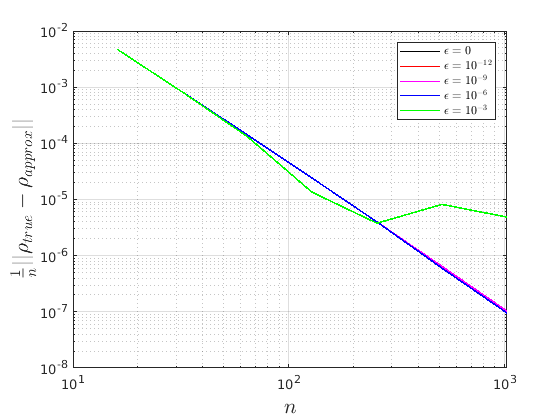
\includegraphics[scale=0.5]{convergence.png}
  \end{figure}
\end{frame}

\begin{frame}{Outlook}
  \begin{itemize}
    \item develop performance study for effect of filling factor on time to
          solution, overheads... with and without wavelet scheme
    \item weakly compressible turbulence (uniform mesh)
    \item compressible turbulence (potentially adaptive)
    \item turbulent combustion (adaptive)
  \end{itemize}
\end{frame}
  
\begin{frame}{Turbulence}
  \begin{figure}
    \center
    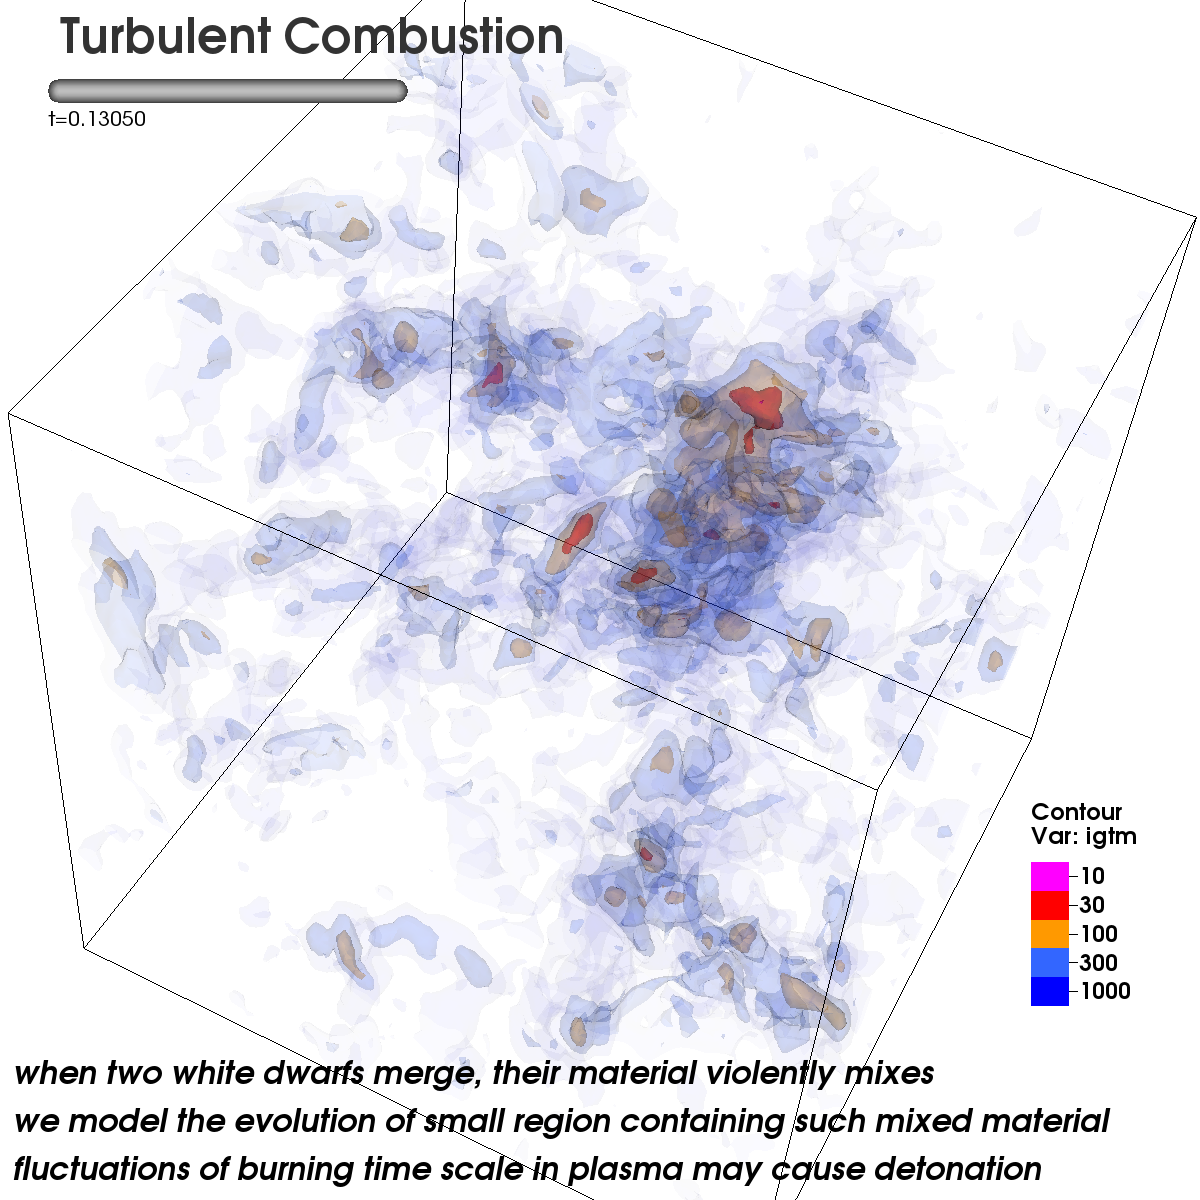
\includegraphics[scale=0.15]{tburn1.png}
  \end{figure}
\end{frame}

\end{document}
